\chapter{Docker}
\label{c:docker}
Zu Beginn ist es notwendig, die Grundlagen von Docker zu verstehen. Hierfür bietet dieses Kapitel einen Einblick in die wichtigsten Begrifflichkeiten, die Architektur und die für diese Arbeit notwendigen Funktionalitäten.
\section{Einführung in Docker}
\label{c:einführung}
\begin{figure}
	\centering
	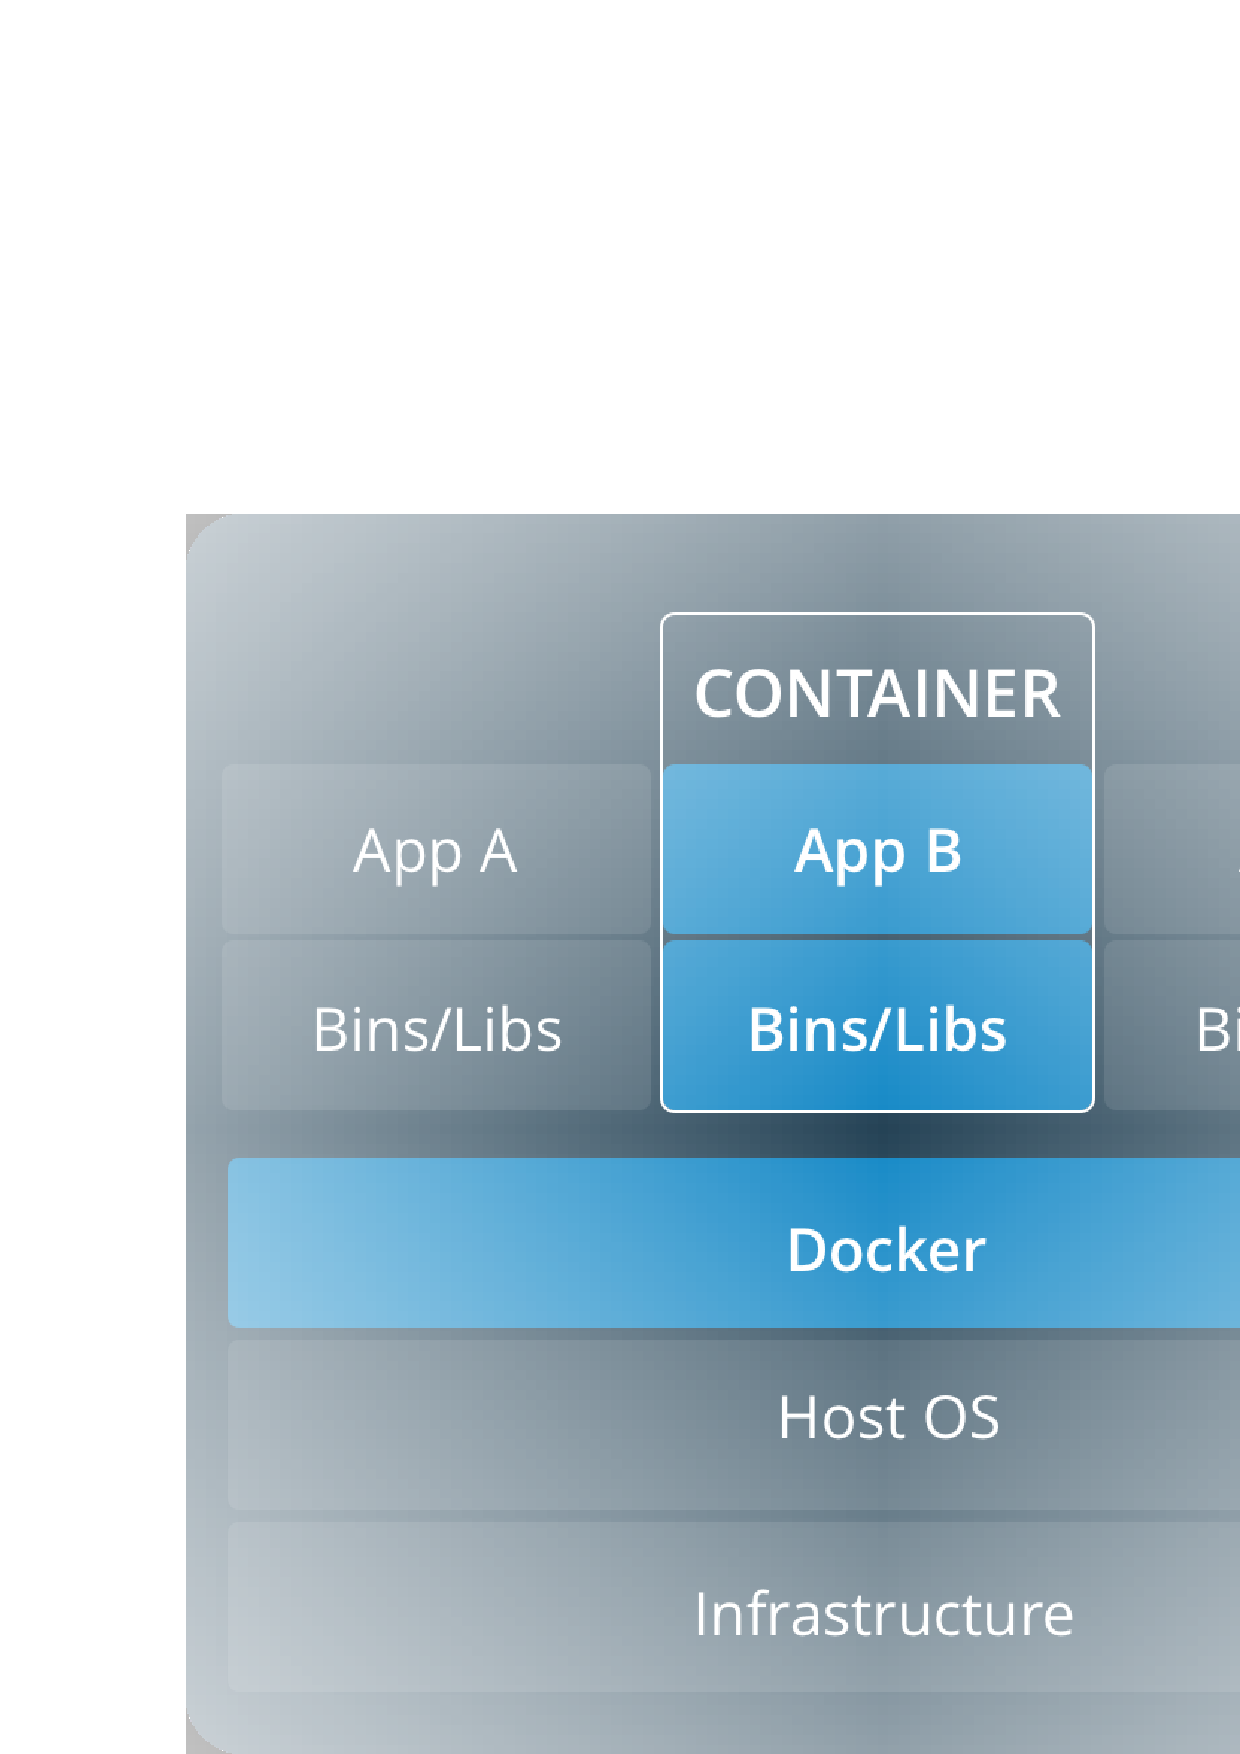
\includegraphics[width=0.7\linewidth]{figures/Docker}
	\caption[Betriebssystem Virtualisierung mit Docker-Containern]{Umsetzung einer Betriebssystem basierten Virtualisierung mit Docker-Containern}
	\label{fig:docker}
\end{figure}
\begin{figure}
	\centering
	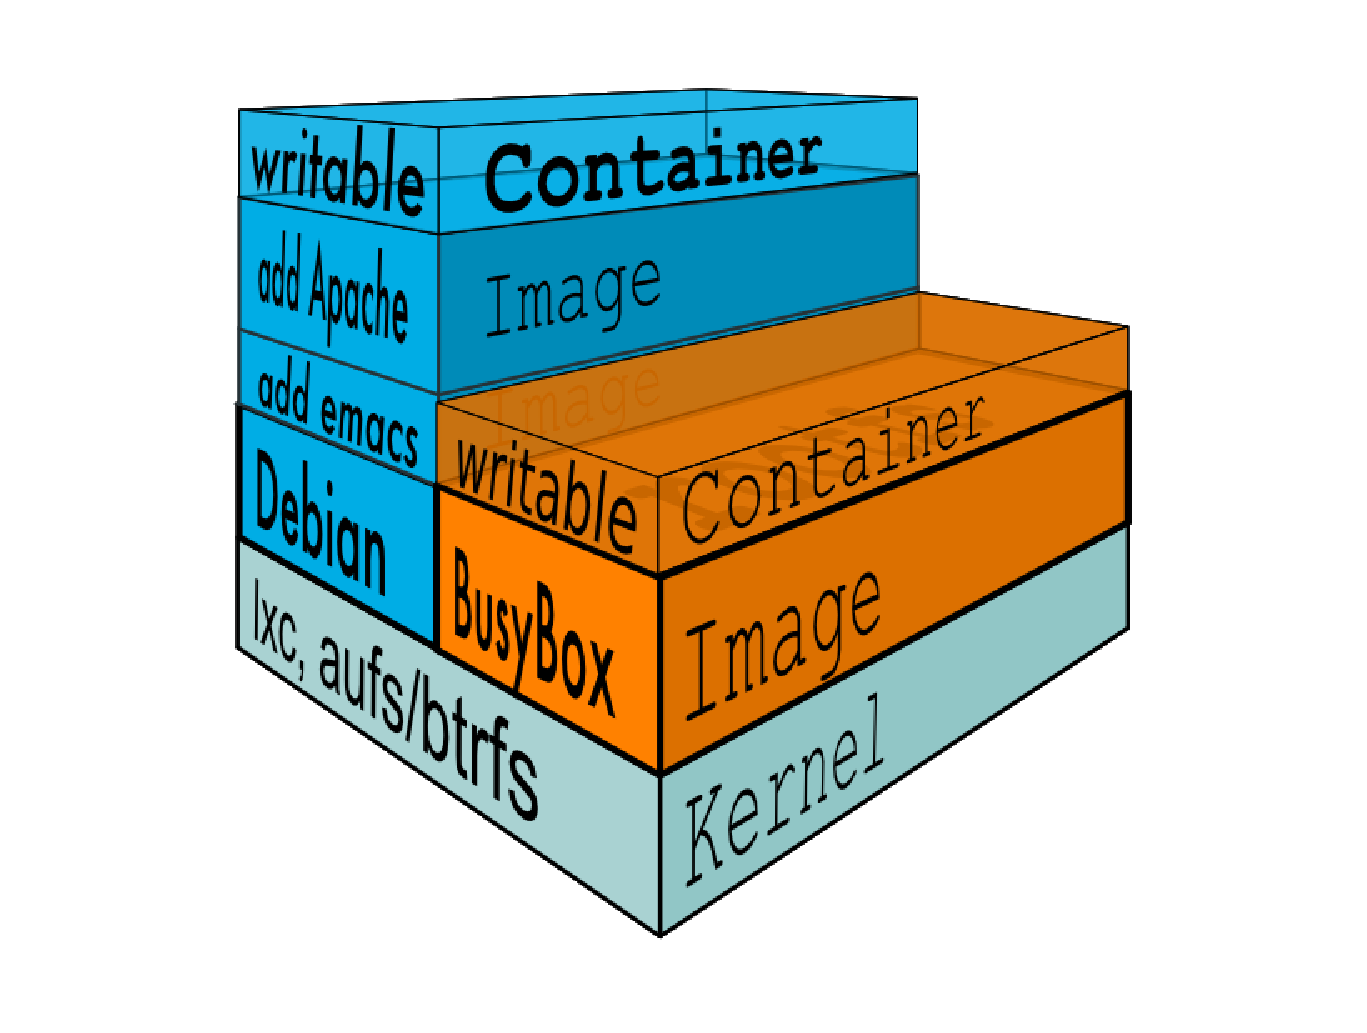
\includegraphics[width=0.7\linewidth]{figures/DockerLayer}
	\caption[Aufbau von Docker mittels Schichten]{Aufbau von Docker mittels Schichten}
	\label{fig:dockerlayer}
\end{figure}
Bei Docker handelt es sich um eine containerbasierte Virtualisierung. Es ist möglich, die Docker-Container sowohl auf einem Windows-System, Unix-System, in der Cloud oder sogar in einer virtuellen Maschine auszuführen. Hierfür wird, wie in Abbildung \ref{fig:docker} gezeigt, in einem Host Betriebssystem die Docker Runtime zur Verfügung gestellt sowie mehrere Docker-Container ausgeführt. Die Docker Runtime übernimmt die Verwaltung der einzelnen Docker-Container, die die benötigten Binaries, Bibliotheken und Anwendungen enthalten. 
\\\\
Im Vergleich zur Virtualisierung mittels einer virtuellen Maschine (VM) bieten Docker-Container einige Vorteile. Hierzu zählen einerseits der geringere Bedarf an CPU, RAM und Speicher sowie andererseits die schnelle Startgeschwindigkeit eines Docker-Containers im Vergleich zu einer herkömmlichen VM.
\\\\
Trotz dessen, dass sich die Docker Container, wie in Abbildung \ref{fig:docker} abgebildet, ein Betriebssystemkernel teilen, sind diese vollständig voneinander isoliert, was dazu führt, dass sich Docker-Container besonders für continuous Integration und Development eignen. Dies ist möglich, da die Workspaces, in Docker Container genannt, auf Linux Containern basieren und somit zur Isolierung die folgenden Namespaces genutzt werden:
\begin{itemize}
	\item ipc-Namespace zur Verwaltung der Interprozess Kommunikationsressourcen (shared Memory)
	\item mnt-Namespace zur Verwaltung des Dateisystems
	\item net-Namespace zur Verwaltung des Netzwerk Interfaces
	\item pid-Namespace zur Isolation von Prozessen
	\item uts-Namespace zur Isolation des Kernels und der Versions Identifier
\end{itemize}
Zur Kontrolle der Hardware Ressourcen verwendet Docker die von Linux stammenden control groups (cgroups). Mittels diesen ist es möglich, den Containern Hardware Ressourcen zuzuweisen und diese nötigenfalls wie z. B. den RAM zu beschränken.
\\\\
Neben den oben genannten Funktionen nutzt Docker mit dem Union file system (UnionFS) eine weitere Linux Funktion. Hierbei wird, wie in Abbildung \ref{fig:dockerlayer} zu sehen, auf dem Boot Dateisystem (Kernel) ein Dateisystem Stack erzeugt, der aus mehreren read only Layern, die Images genannt werden, besteht. Jedes Image referenziert und beinhaltet lediglich Ergänzungen zum vorherigen Image. Dies macht Docker leichtgewichtig und schnell und ermöglicht einen hohen Workload auf der gleichen Hardware.
\\\\
Beim Start von Docker wird, wie in Abbildung \ref{fig:dockerlayer} dargestellt, ein read-write Container auf dem Stack erzeugt. In diesem werden die notwendigen Dateien der darunterliegenden Images kopiert und dort nötigenfalls umgeschrieben und abgelegt. Wird Docker gestoppt, so werden einerseits der writable Container und andererseits sämtliche Änderungen an den Dateien, falls nicht ein Speichervolumen außerhalb des UnionFS angebunden wurde, gelöscht. Somit ist es möglich, die Docker-Container immer zu den gleichen Bedingungen zu starten.
\section{Architektur}
\label{c:architektur}
Wird die Docker Architektur betrachtet so zeigt die Abbildung \ref{fig:dockerengine}, dass es sich bei der Docker Runtime oder auch Docker-Engine lediglich um eine Client-Server-Architektur mit mehreren Hauptkomponenten handelt.
\\\\
Im Kern der Docker-Engine befindet sich, wie in Abbildung \ref{fig:dockerengine} gezeigt, der Server oder auch Docker Daemon. Dieser erstellt und verwaltet einerseits die Docker-Container, Images, Netzwerke und Dateisysteme und er ist andererseits in der Lage, mit anderen Docker Daemons zu kommunizieren. Mittels einer REST-API und dem command line interface (CLI) ist der Client im Stande, mit einem oder mehreren Docker Daemons zu interagieren und diesen, per CLI Kommandos oder mit Hilfe von Skripten, Aufträge zu erteilen.
\\\\
Ein weiterer wichtiger Bestandteil der Docker Architektur sind, wie in Abbildung \ref{fig:dockerarchitecture} zu sehen, die Docker Registries. Hierbei wird zwischen privaten und öffentlichen Registries unterschieden. Die wichtigsten öffentlichen Registries sind der Docker Hub und die Docker Cloud. So wird z. B. mittels der Befehle docker run oder docker pull per default das Standard Dockerfile vom Docker Hub genutzt, um einerseits die Standard images und andererseits den Container über dem Dateisystem Stack automatisch zu bauen. Hierfür enthält das Dockerfile alle notwendigen Kommandos.
\\\\
Des Weiteren besteht die Möglichkeit, mit Hilfe des Docker Datacenter (DDC) eigene (private) Registries anzulegen und z. B. mittels des docker push Kommandos eigene Dockerfiles in den neu angelegten Registries abzulegen und später für den Buildprozess zu nutzen.
\begin{figure}
	\centering
	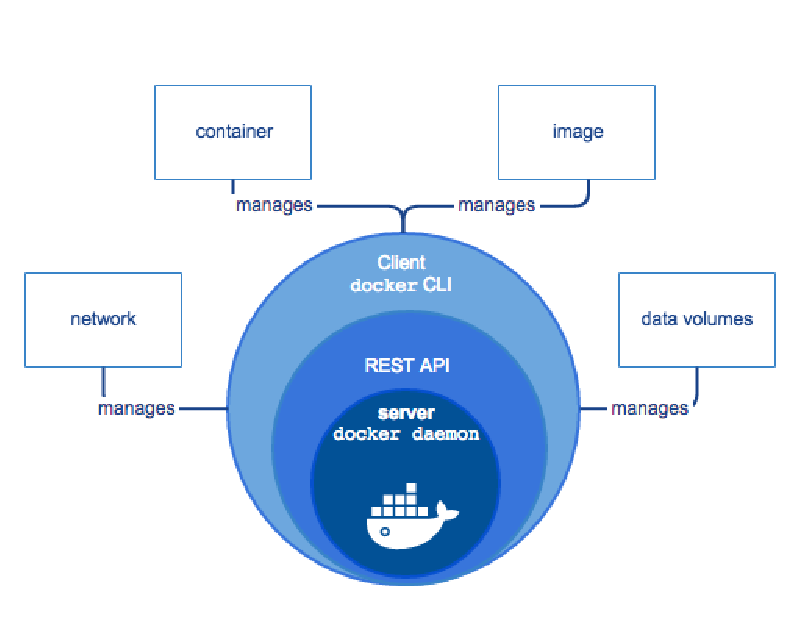
\includegraphics[width=0.7\linewidth]{figures/DockerEngine}
	\caption[Aufbau Docker-Engine]{Schematische Darstellung des Aufbaus der Docker-Engine}
	\label{fig:dockerengine}
\end{figure}
\begin{figure}
	\centering
	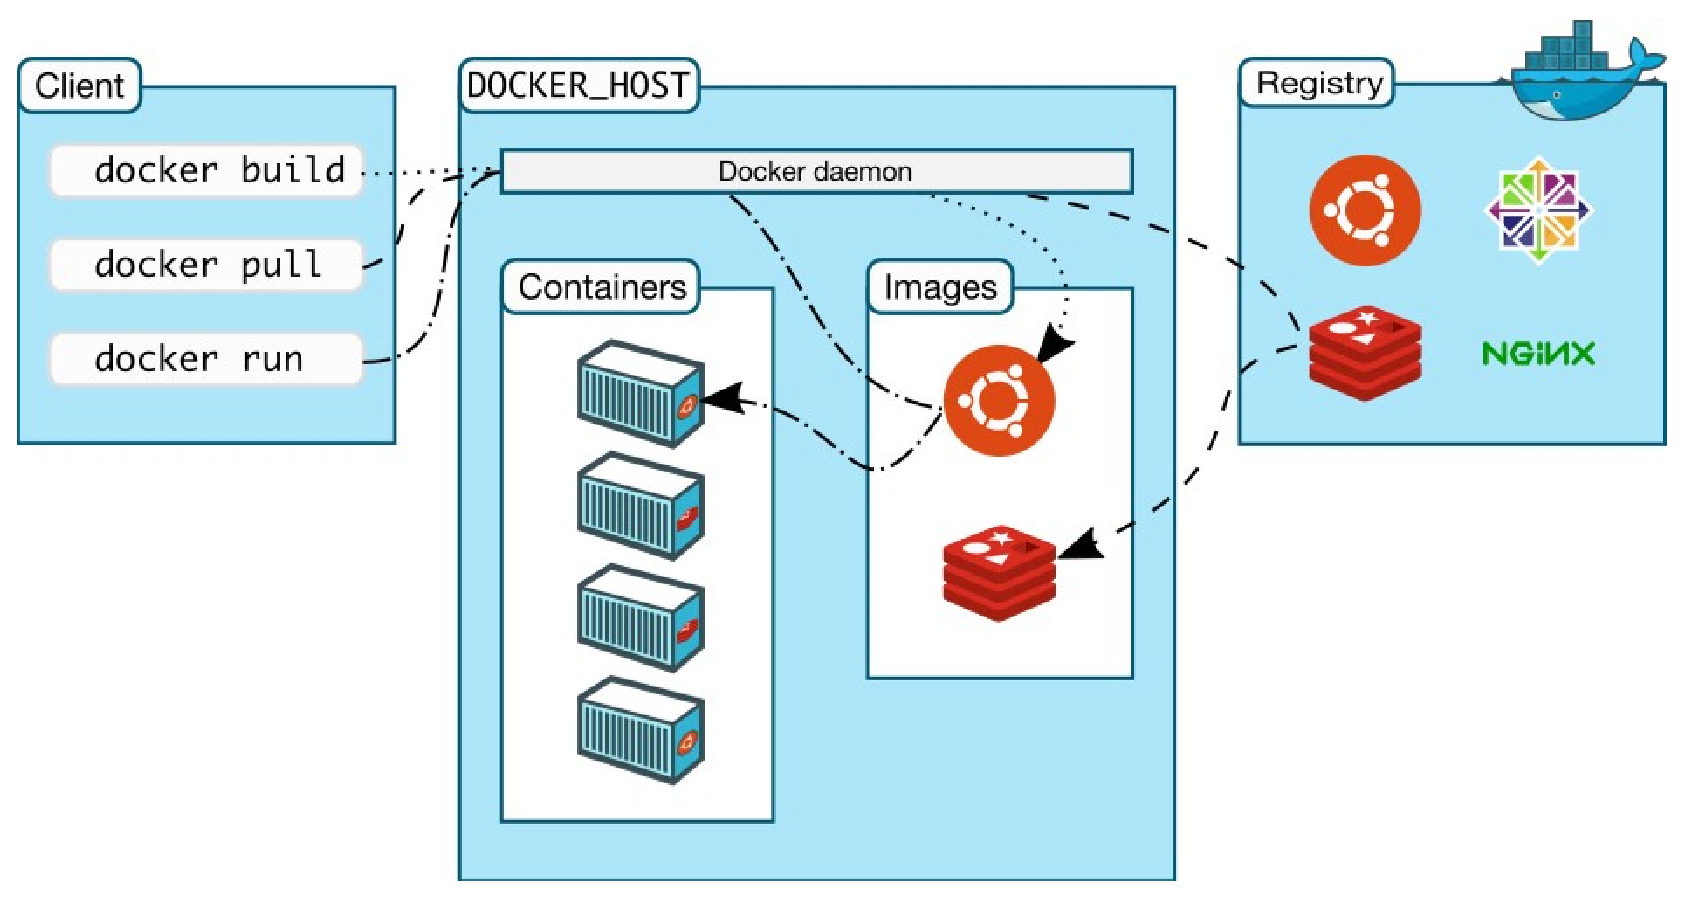
\includegraphics[width=0.7\linewidth]{figures/DockerArchitecture}
	\caption[Detailansicht der Docker-Architektur]{Detailansicht der Docker-Architektur}
	\label{fig:dockerarchitecture}
\end{figure}
\section{Docker Funktionalitäten}
\label{c:funktionalität}
Im folgenden Unterkapitel werden die, für diese Arbeit wichtigsten Docker Funktionalitäten erläutert. Hierbei wird falls notwendig anhand einer Begründung erklärt, weshalb eine bestimmte Ausprägung einer Funktionalität gewählt wurde.
\subsection{Docker Compose}
Standardmäßig wird jeder Docker-Container einzeln mit dem Kommando docker run gestartet und ausgeführt. Betrachtet man den Titel dieser Arbeit, "Containers with Machine Guns", so geht daraus hervor, dass es sich nicht zwingend um einen einzelnen Container handelt, sondern möglicherweise um eine Vielzahl von Containern. Diese sollen nach Möglichkeit alle gleichzeitig gestartet und ausgeführt werden.
\\\\
Um dies zu erreichen, bietet Docker Compose an. Hierbei handelt es sich um ein Tool von Docker, mit dem es möglich ist, einen Service für eine Anwendung zu konfigurieren und diese sowie die dazugehörigen Container anschließend mit einem einzigen Befehl zu starten.
\\\\
Hierfür wird zu Beginn ein Dockerfile erstellt, mit dem es möglich ist, die Images und Container einfach zu vervielfältigen. Im Anschluss daran wird die YAML-Datei docker-compose.yml genutzt, um den Service zu definieren. Code-Beispiel \ref{dockerComposeFile} zeigt, wie in dieser Datei z. B. die zwei Services web und redis definiert werden. Des Weiteren wird dargestellt, wie der Service web im Punkt build das Dockerfile aus dem aktuellen Verzeichnis und der Service redis das öffentliche Redis image "redis:alpine" des Docker Hub verwendet. Zusätzlich ist ersichtlich, dass der Service web über den default port 5000 des Flask web servers erreichbar ist. Mittels des Kommandos docker-compose up wird anschließend die gesamte Anwendung anhand der Compose-Datei gestartet.
\\\\
\begin{minipage}{\linewidth}
	\begin{lstlisting}[frame=single,caption=Beispiel Docker Compose Datei, label=dockerComposeFile, language=Scala]
	version: '3'
	services:
	  web:
	    build: .
	    ports:
	     - "5000:5000"
	  redis:
	    image: "redis:alpine"
	\end{lstlisting}
\end{minipage}
\\\\
Mit Hilfe von Compose ist es neben dem Starten des Service, möglich, diesen zu stoppen, erneut zu bauen und Befehle an einzelne Container des Service zu senden. Des Weiteren ermöglicht Compose die Statusabfrage sowie das Auslesen von Logs eines laufenden Service.
\subsection{Netzwerke}
Dieser Abschnitt des Kapitels zeigt die default Netzwerke und die Möglichkeiten zum Definieren eines eigenen Netzwerkes in Docker auf. Hiermit soll erläutert werden, wie der angelegte Service von außerhalb des Host-Systems verfügbar gemacht wird.
\subsubsection{Default Netzwerke}
Mit der Installation von Docker werden standardmäßig die folgenden drei Netzwerke erzeugt:
\begin{itemize}
	\item None-Netzwerk
	\item Host-Netzwerk
	\item Bridge-Netzwerk
\end{itemize}
Das None-Netzwerk ermöglicht es, einen Container zu einem spezifischen Netzwerk Stack hinzuzufügen, allerdings besitzt dieser Container kein eigenes Netzwerk-Interface. 
\\\\
Mit Hilfe des Host-Netzwerkes wird der Container zum Netzwerk Stack des Host Systems hinzugefügt. Dies hat zur Folge, dass keine Isolation zwischen dem Host System und den Containern mehr gegeben ist. Des Weiteren sind sowohl das None als auch das Host-Netzwerk nicht direkt mit Docker konfigurierbar.
\\\\
Das dritte default Netzwerk, das Bridge-Netzwerk, ist auf allen Host Systemen von Docker vorhanden. Wird kein alternatives Netzwerk definiert, so wird jeder neu erstellte Container automatisch an dieses gekoppelt. Die angebundenen Container wären zwar per Port Mapping und mit Hilfe von IP-Adressen, aber nicht mit den Containernamen per DNS-Auflösung, in der Lage miteinander zu kommunizieren, aber dieses Vorgehen wird für das default Bridge-Netzwerk von Docker nicht empfohlen. Stattdessen sollte für derartige Anwendungsfälle das, im Abschnitt User definierte Netzwerke, beschriebene Bridge-Netzwerk verwendet werden.
\subsubsection{User definierte Netzwerke}
Zur Erstellung eines User definierten Netzwerks bietet Docker entsprechende Treiber an. Mit diesen ist es möglich, die folgenden Netzwerke anzulegen:
\begin{itemize}
	\item User definierte Bridge-Netzwerke
	\item Overlay-Netzwerke
	\item MACVLAN-Netzwerke
\end{itemize}
Wenn keines der gelisteten Netzwerke dem Anwendungsfall entspricht, so besteht die Möglichkeit, ein eigenes Plugin für einen Netzwerk-Treiber zu erstellen. Eine genau Beschreibung hierfür sowie für das oben gelistete MACVLAN-Netzwerk würde für diese Arbeit zu weit gehen, weshalb diese an dieser Stelle nur zum Zweck der Vollständigkeit erwähnt werden.
\\\\
Das User definierte Bridge-Netzwerk bietet mit Hilfe des eingebetteten DNS-Server, des Docker Daemon, eine DNS-Auflösung. Des Weiteren besteht optional die Möglichkeit zur Steuerung der Kommunikation der sich auf einem Host-System und in einem Netzwerk befindlichen Container. Diese können an kein oder jederzeit, auch während der Ausführung eines Containers, an ein oder mehrere Netzwerke angeschlossen oder von diesen getrennt werden. Ist dies nicht erforderlich, so sind alle Container ohne weitere Konfiguration in der Lage, mit jedem beliebigen Container des Netzwerkes zu kommunizieren. Hieraus geht hervor, dass das Netzwerk die darin befindlichen Container vollständig, wie in Abbildung \ref{fig:dockerportpuex} zu sehen, isoliert.
\begin{figure}
	\centering
	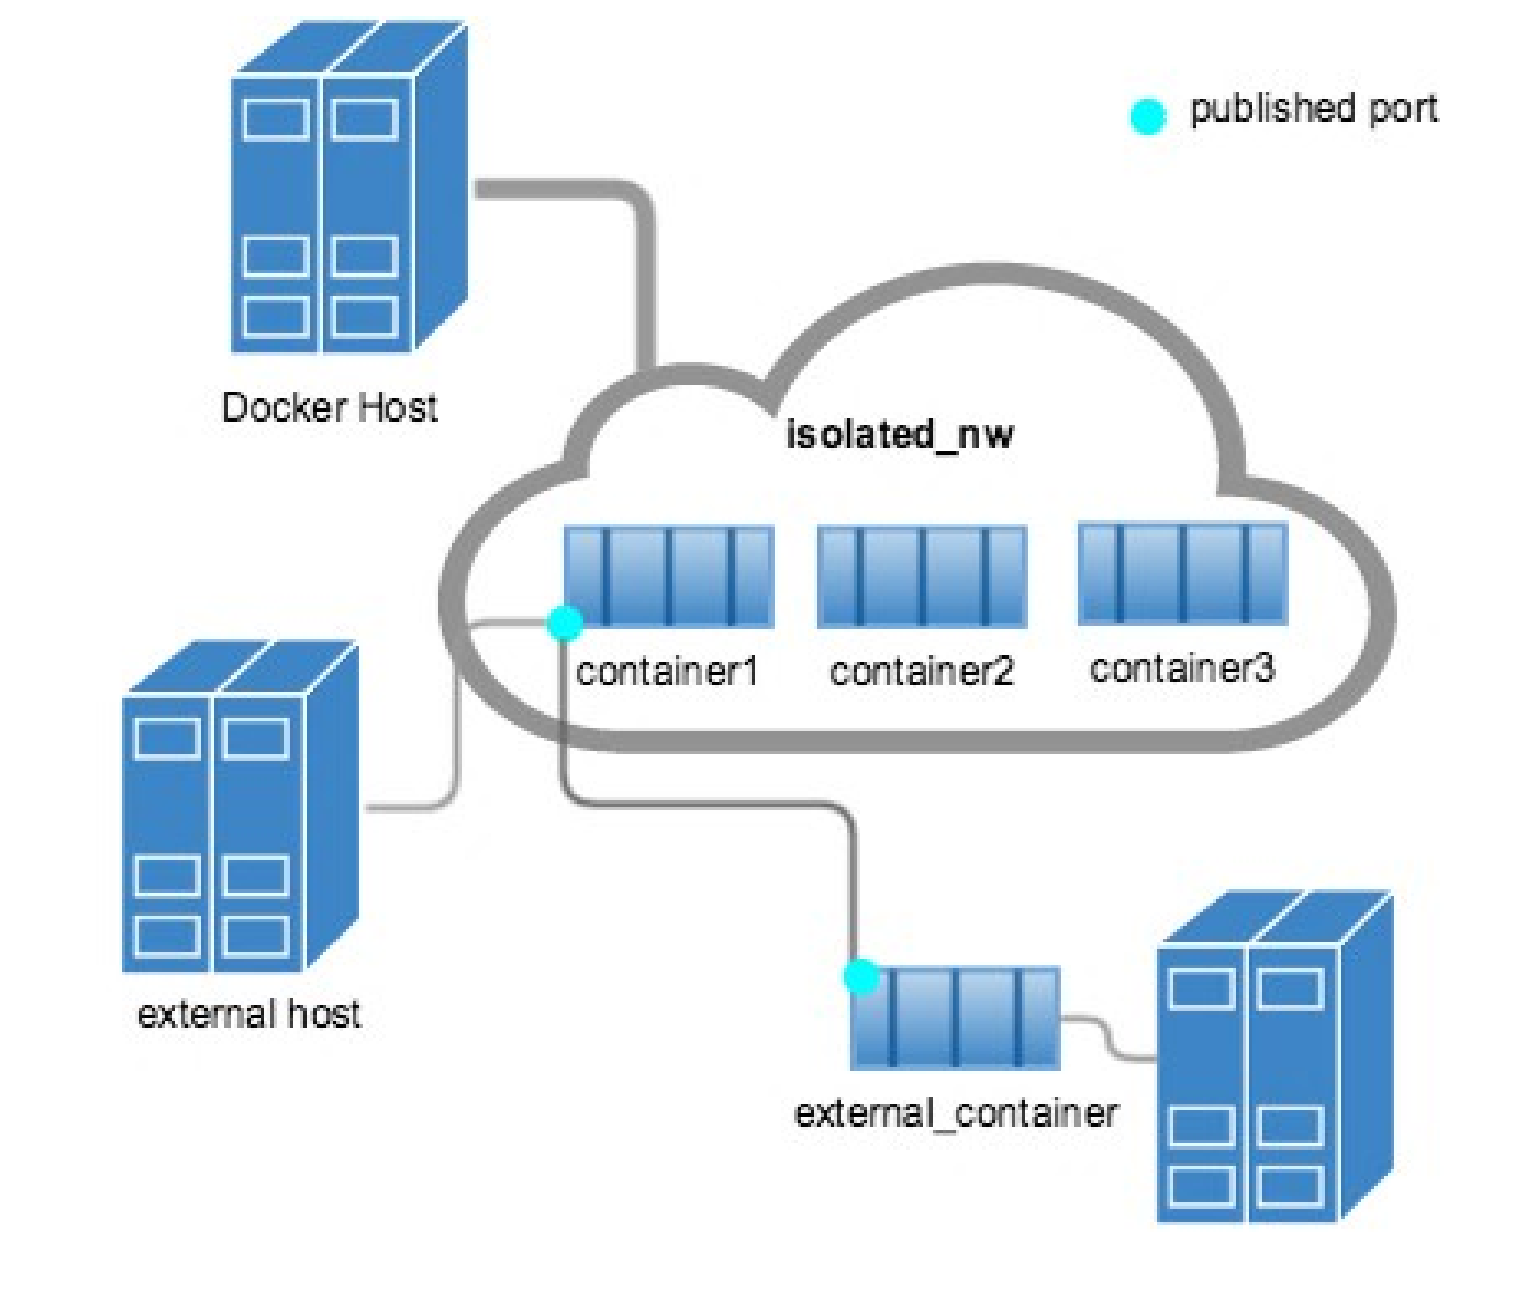
\includegraphics[width=0.7\linewidth]{figures/DockerPortPuEx}
	\caption[Docker Netzwerkzugriff]{Diagramm zur Darstellung des Docker Netzwerkzugriffs im User definierten Bridge-Netzwerk}
	\label{fig:dockerportpuex}
\end{figure}
\\\\
Möchte man nun in einem default oder User definierten Bridge-Netzwerk eines Host-Systems, wie in Abbildung \ref{fig:dockerportpuex} abgebildet, dass z. B. einzelne Container sich mit einem externem Host oder einem externen Container austauschen können, so ist ein Port exposing und publishing notwendig. Das Port exposing erfolgt entweder durch Eintragung einer beliebigen Portnummer in Kombination mit dem Schlüsselwort EXPOSE im Dockerfile oder durch Ergänzung des docker run Kommandos mit dem Flag - -expose.
\\\\
Für das publishing ist das Festlegen eines Ports im Dockerfile nicht möglich. Stattdessen wird das docker run Kommando durch das Flag - -publish oder - -publish-all ergänzt. Dies teilt mit, welcher Port > 30000 auf dem Host-System verfügbar ist. Möchte man dennoch einen speziellen Port verwenden, so ist die Zuweisung des Ports erst zur Laufzeit möglich.
\\\\
Aufgrund dessen, dass User definierte Bridge-Netzwerke vorrangig dafür verwendet werden kleinere Netzwerke auf einem Host zu erstellen, eignet sich diese Netzwerklösung nicht zur Umsetzung des Themas. Dies liegt daran, dass Docker für diese Arbeit im Swarm Modus genutzt wird. Hierbei handelt es sich um ein Cluster aus mehreren Docker Engines. Das Cluster besitzt mindestens einen Swarm-Manager. Dieser nimmt Befehle für den Swarm entgegen und ermöglicht es, neue Swarm-Nodes oder auch Swarm-Worker genannt, aber keine einzelnen Docker-Container zum Cluster hinzuzufügen.
\\\\
Statt des User definierten Bridge-Netzwerks bietet Docker hierfür die Möglichkeit zur Erstellung eines Overlay-Netzwerks auf einem Swarm-Manager an. Hierbei wird automatisch die Netzwerkbrücke docker\_gwbridge, die zur Kommunikation zwischen den Swarm-Nodes verwendet wird, erstellt. Diese Netzwerkbrücke wird zusätzlich immer dann angelegt, wenn ein gewöhnlicher Docker Container keine Anbindung an ein externes Netz besitzt. Der Swarm-Manager gewährt den einzelnen Swarm-Workern immer dann den Zugriff auf das Netzwerk, wenn die Swarm-Worker das Netzwerk zur Bewältigung ihrer Aufgaben benötigen. 
\\\\
Bei der Erstellung des Overlay-Netzwerks ist zu beachten, dass die Docker Engine im Swarm Modus arbeitet und der gewählte Swarm-Manager nicht an einen externen Key-Value-Store wie, z. B. ZooKeeper, angebunden ist.
\\\\
Andernfalls spricht man von einem Overlay-Netzwerk ohne Swarm Modus. Dieses wird in dieser Arbeit nicht weiter erläutert. Einerseits, da es nicht erforderlich ist und andererseits, da Docker hierzu folgenden Satz in ihrem Docker container networking Guide verfasste:
\begin{quote}
	\textit{\grqq It may be deprecated in the future. \grqq}
\end{quote}
\subsection{Volumes und shared Volumes}
